\section{Laboratory work implementation}

\subsection{Tasks and Points}

I chose to implement the tasks for \textit{Advanced Level}:
\begin{enumerate}
	\item Create a Windows application what will display a dialog box on some event (ex. on clicking some button)
    \item Add a system menu to your application with at least 3 items (add actions to that items)
    \item Hook keyboard input. Add 2 custom events for 2 different keyboard combinations (ex. change window background on ctrl+space)
	\item Add a scroll bar that will change any visible parameter of any other element (color of a text) OR other 2 scroll bars that will manage main window size or position
    \item Customize your application by adding an icon and using different cursor in application
    \item Add a listbox and attach some events when any element is accessed (clicked) 
    \item \textit{Bonus Task}:Use a scroll bar to scroll through application working space. Scroll should appear only when necessary (eg. when window width is smaller than 300px)
\end{enumerate}

\subsection{Laboratory work analysis}

 \url{https://github.com/szraksy/WP}

I made 2 different forms on my Second Labrotary work. First form has
custom background image ,listbox which one is represent to the Education
year , a button and a message box.
We are chosing the year of the education from the listbox and we are
clicking to the button when we clicked to the button then message box
appeare and it is saying which year we chosed.
When we click to the Ok on the message box then the second form will be
open.
On the second form we have 5 different menu items, announcement area
with listbox ,a button, a label ,
on the menu side we have 5 different options which are;
\begin{enumerate}
	\item Changing background color
	\item changing window size
	\item changing background color of Button
	\item Reseting to the default color
	\item and exit from the program
\end{enumerate}

When we are clicking to the button then we will see more announcements and the
listbox’s scrollbar will be visible.
On my program i put custom icon.
	



\subsection{Prove your work with screens}

\begin{figure}
	\centering
	
\includegraphics[width=0.7\linewidth]{form1}
	\caption{}
	\label{fig:form1}
\end{figure}

\begin{figure}
	\centering
	
\includegraphics[width=0.7\linewidth]{form1-2}
	\caption{}
	\label{fig:form1-2}
\end{figure}


\begin{figure}
	\centering
	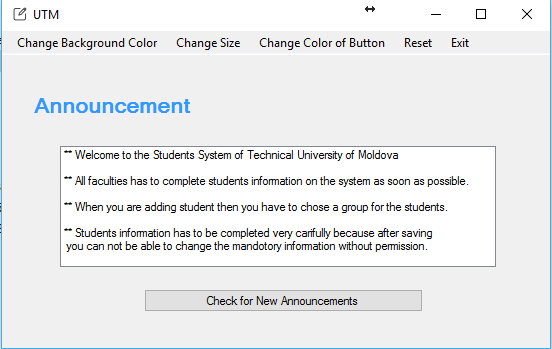
\includegraphics[width=0.7\linewidth]{form2}
	\caption{}
	\label{fig:form2}
\end{figure}


\begin{figure}
	\centering
	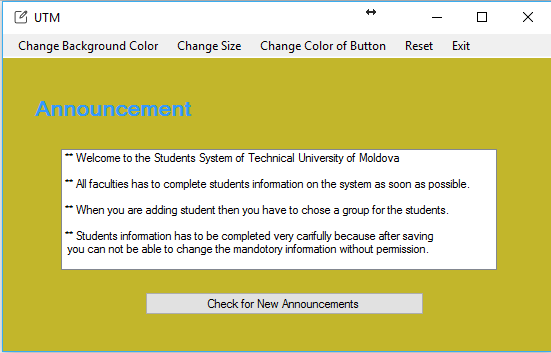
\includegraphics[width=0.7\linewidth]{form2-2}
	\caption{}
	\label{fig:form2-2}
\end{figure}


\begin{figure}
	\centering
	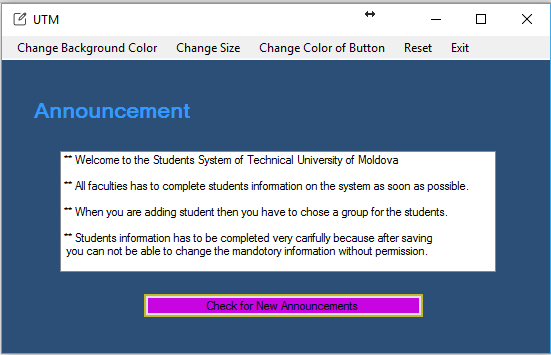
\includegraphics[width=0.7\linewidth]{form2-3}
	\caption{}
	\label{fig:form2-3}
\end{figure}


\begin{figure}
	\centering
	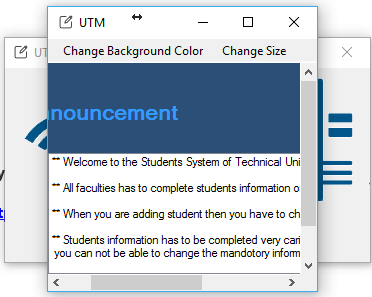
\includegraphics[width=0.7\linewidth]{form2-4}
	\caption{}
	\label{fig:form2-4}
\end{figure}


\clearpage